\chapter{MARCO TEÓRICO} 
	
	\vspace{0pt}
	
	\section{LOGÍSTICA DEL TRANSPORTE DE PASAJEROS}
	\subsection{Logística}
		``Logística es planificar, operar, controlar y detectar oportunidades de mejora del proceso de flujo de materiales (insumos, productos), servicios, información y dinero.  Es la función que normalmente opera como nexo entre las fuentes de aporvisionamiento y suministro y el cliente final o la distribución.  Su objetivo es satisfacer permanentemente la demanda en cuanto a cantidad, oportunidad y calidad al menor costo posible para la empresa.''\parencite{carro2013logistica}
	\subsection{Transporte}
	
	\subsection{Sistema de transporte}
	\subsection{Funcionalidad del transporte}
	\section{RESERVA Y VENTA DE PASAJES}
	\subsection{Proceso de reserva y venta de pasajes}
	\subsection{Emisión y gestion de boletos}
	\subsection{Cambios y cancelaciones}
	\section{SERVICIO DE TRANSPORTE DE PASAJEROS Y ENCOMIENDAS}
	\section{LOGÍSTICA DE ENVÍO DE ENCOMIENDAS}
	\subsection{Encomienda}
	\subsection{Proceso de recepción}
	\subsection{Clasificación de encomiendas}
	\subsection{Embalaje y etiquetado}
	\subsection{Entrega al destinatario}
	\section{GESTIÓN DE BUSES}
	\subsection{Asignación de rutas}
	\subsection{Análisis y demanda de pasajeros}
	\subsection{Programación y asignación de conductores}
	
	
		
	%\vspace{0.3cm} % Agregar 1 cm de espacio entre el párrafo y la figura
		
	%	\begin{figure}[h] % 'H' del paquete 'float' para mantener posición	
	%		\caption[Descripción corta]
	%		{\newline Resultados del informe PISA 2022.} % Leyenda en la parte superior
	%		\centering
	%		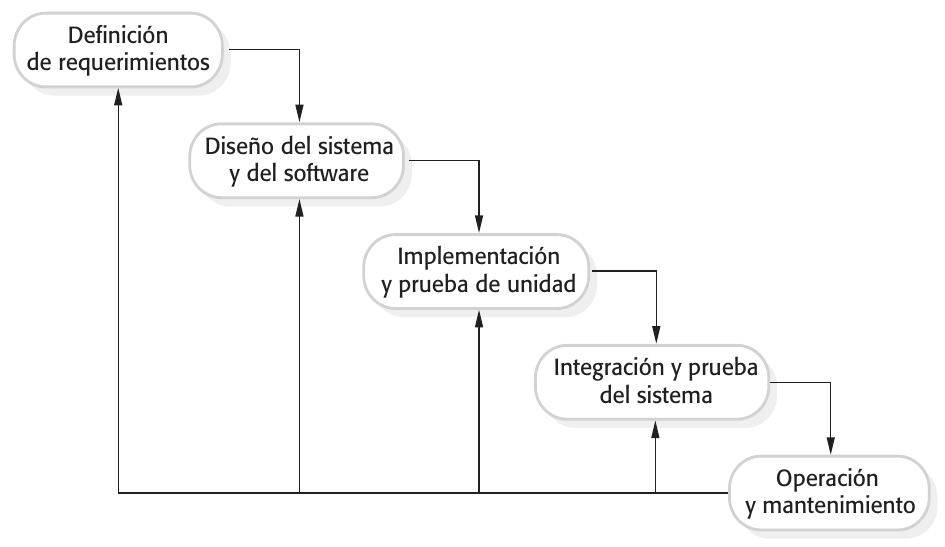
\includegraphics[width=0.95\textwidth]{imagenes/figura2_1.png} % Inserta una imagen
	%		
	%		\begin{flushleft}
	%			\hspace{1.20cm} \textit{Nota.} al pie asociada con esta figura, explicando detalles adicionales. % Nota al pie para esta figura
	%		\end{flushleft}
	%		\vspace{-16pt}
	%		\label{fig:figura2_1} % Etiqueta para referencia cruzada
	%	\end{figure}

	
	
	\section{MARCO LEGAL Y NORMATIVO}
	\subsection{Autoridad de regulación y fiscalización de telecomunicaciones y transportes}
	\subsection{Ley general del transporte}
	\subsection{Reglamento regulatorio de transporte terrestre}


